\documentclass[12pt,a4paper]{article}

% To use this template make changes to following:
% 1. Fill-ables section.
% 2. Instructions.
% 3. Marks table.
% 4. Actual questions.

% ================================ 1. Fill-ables ================================
\newcommand\University{National University of Computer and Emerging Sciences}
\newcommand\Department{School of Engineering}
\newcommand\Campus{Islamabad Campus}
\newcommand\Semester{Spring 2014}
\newcommand\Exam{Final Exam}
\newcommand\Subject{NS110--Physics for Engineers}
\newcommand\ExamDate{Friday, May 16, 2014}
\newcommand\InstructorOne{Instructor 1}
\newcommand\InstructorTwo{Instructor 2}
\newcommand\InstructorThree{\null}
\newcommand\TotalTime{03 Hours}
\newcommand\TotalMarks{135}
\newcommand\TotalQuestions{10}
\newcommand\TotalPages{\pageref{LastPage}} % Automatic: No need to change this.
% Marks of each question
\def\Qone{5}
\def\Qtwo{15}
\def\Qthree{10}
\def\Qfour{20}
\def\Qfive{10}
\def\Qsix{10}
\def\Qseven{10}
\def\Qeight{27}
\def\Qnine{11}
\def\Qten{17}
% ============================================================================

% ============== 2. Packages ==============
\usepackage{amsmath}
\usepackage{float}
\usepackage{graphicx}
\usepackage[hyphens]{url}
\usepackage[hidelinks]{hyperref}	% Clickable links to figures, references and urls.
\usepackage{lastpage}
\usepackage{array}
\usepackage{fancyhdr}
\usepackage{afterpage}
% Drawing packages.
\usepackage{pgf}
\usepackage{tikz}
% Listings for formatting code.
\usepackage{listings}
\usepackage{textcomp}

% General listings options.
\lstset{breaklines=true, basicstyle=\footnotesize\ttfamily, tabsize=4, numbers=left, stepnumber=1, frame=none, showstringspaces=false, upquote=true}
% C++ specific high-lighting. Comments are 50/50 shades of green/black and strings coloured with 60/40 red/black mixture.
\lstset{language=[ISO]C++, commentstyle=\color{green!50!black}, keywordstyle=\color{blue}, stringstyle=\color{red!60!black}}

% Table cell alignment directives.
\newcolumntype{L}[1]{>{\raggedright\let\newline\\\arraybackslash\hspace{0pt}}m{#1}}
\newcolumntype{C}[1]{>{\centering\let\newline\\\arraybackslash\hspace{0pt}}m{#1}}
\newcolumntype{R}[1]{>{\raggedleft\let\newline\\\arraybackslash\hspace{0pt}}m{#1}}

% Line spacing.
\def\SingleSpacing{\def\baselinestretch{1}\large\normalsize}
\def\DoubleSpacing{\def\baselinestretch{1.5}\large\normalsize}

% Margins.
\setlength{\oddsidemargin}{0in}
\setlength{\evensidemargin}{0in}
\setlength{\headheight}{28pt}
\setlength{\headsep}{2.5pt}
\setlength{\topmargin}{-60pt}
\setlength{\textwidth}{6.5in}
\setlength{\textheight}{10.75in} % Actual: 10.75in

% ============================= 3. Header and Footer ============================
\pagestyle{empty}
% Header
\chead
{
	{\large\textbf{\University}}\\
	\begin{minipage}{0.45\textwidth}
	\begin{center}
	{\small\textbf{\Department}}
	\end{center}
	\end{minipage}
	\begin{minipage}{0.45\textwidth}
	\begin{center}
	{\small\textbf{\Campus}}
	\end{center}
	\end{minipage}
}
% Footer
\lfoot{{\small\Exam}}
\cfoot{{\small\Semester}}
\rfoot{{\small Page \textbf{\thepage}~of \textbf{\TotalPages}}}
\renewcommand{\headrulewidth}{0.4pt}
\renewcommand{\footrulewidth}{0.4pt}
% ================================= 4. Front Page ===============================
\begin{document}
% A cute macro to add up marks of all individual questions. Uncomment if you want to use this.
%\pgfmathtruncatemacro\TotalMarks{\Qone+\Qtwo+\Qthree+\Qfour+\Qfive+\Qsix+\Qseven+\Qeight+\Qnine+\Qten}
% Use this macro if marks are in decimal points
%\newcommand\TotalMarks{\pgfmathsetmacro\TotalMarks{\Qone+\Qtwo+\Qthree+\Qfour+\Qfive+\Qsix+\Qseven+\Qeight+\Qnine+\Qten}}
\begin{minipage}[t]{0.6\textwidth}
\begin{flushleft}
\DoubleSpacing
{\Large\textbf{\Subject}}\\
{\normalsize\ExamDate}\\
{\large\textbf{Course Instructor}}\\
{\normalsize\InstructorOne}\\
{\normalsize\InstructorTwo}\\
{\normalsize\InstructorThree}
\end{flushleft}
\end{minipage}
\begin{minipage}[t]{0.01\textwidth}
~
\end{minipage}
\begin{minipage}[t]{0.325\textwidth}
\DoubleSpacing
{\normalsize Serial No:}\\
{\Large\textbf{\Exam}}\\
{\large\textbf{Total Time: \TotalTime}}\\
{\large\textbf{Total Marks: \TotalMarks}}\\[1cm]
\rule{5cm}{0.2mm}\\[-0.25cm]
{\small Signature of Invigilator}
\end{minipage}
\SingleSpacing
~\\[1.5cm] % Extra space.
\rule{7cm}{0.2mm}~\rule{2.5cm}{0.2mm}~\rule{2cm}{0.2mm}~\rule{4.5cm}{0.2mm}\\
{\small Student Name\hspace{4.75cm}Roll No\hspace{1.35cm}Section\hspace{0.95cm}Signature}\\[1cm]
% ============================ 5. Instructions ==================================
\textbf{DO NOT OPEN THE QUESTION BOOK OR START UNTIL INSTRUCTED.}\\
\textbf{Instructions:}
\begin{enumerate}
\itemsep0em
\item Verify at the start of the exam that you have a total of \TotalQuestions~questions printed on \TotalPages~pages including this title page.
\item Attempt all questions on the question-book and in the given order.
\item The exam is closed books, closed notes. Please see that the area in your threshold is free of any material classified as `useful in the paper' or else there may be a charge of cheating.
\item Read the questions carefully for clarity of context and understanding of meaning and make assumptions wherever required, for neither the invigilator will address your queries, nor the teacher/examiner will come to the examination hall for any assistance.
\item Fit in all your answers in the provided space. You may use extra space on the last page if required. If you do so, clearly mark question/part number on that page to avoid confusion. 
\item Use only your own stationery and calculator. If you do not have your own calculator, use manual calculations. 
\item Use only permanent ink-pens. Only the questions attempted with permanent ink-pens will be considered. Any part of paper done in lead pencil cannot be claimed for checking/rechecking.
\item Spend first 30 minutes on Part I; however, if you finish it earlier, you can hand it over and start attempting Part II.
\end{enumerate}
% =============================== 6. Marks Table ================================
\begin{table}[H]
\begin{center}
\vspace{0.3cm}
	{\footnotesize \begin{tabular}{|C{1.8cm}|C{0.75cm}|C{0.75cm}|C{0.75cm}|C{0.75cm}|C{0.75cm}|C{0.75cm}|C{0.75cm}|C{0.75cm}|C{0.75cm}|C{0.75cm}|c|}
	\hline
		\rule{0pt}{4.6ex} & Q-1 & Q-2 & Q-3 & Q-4 & Q-5 & Q-6 & Q-7 & Q-8 & Q-9 & Q-10 & \textbf{Total}\\[-0.5ex]
		\hline
		\rule{0pt}{2.5ex}\textbf{Total Marks}& \Qone & \Qtwo & \Qthree & \Qfour & \Qfive & \Qsix & \Qseven & \Qeight & \Qnine & \Qten & \TotalMarks\\
		\hline
		\rule{0pt}{2.5ex}\textbf{Marks Obtained}& & & & & & & & & & &\\
	\hline
	\end{tabular}}
\end{center}
\end{table}
{\small \textbf{Vetted By: \rule{6cm}{0.2mm} Vetter Signature: \rule{4.5cm}{0.2mm}}}
\setlength{\textheight}{10.5in}
\newpage
\pagestyle{fancy}
% ================================== 7. Questions ===============================
\noindent\textbf{Question 1: Constructors/Destructors \hfill \Qone~marks}\\
Write the output of following program. Mention object name with constructor/destructor calls.
\begin{lstlisting}
#include <iostream>
using namespace std;
class test
{
	public:
	test() { cout << "DC" << endl; }
	test(int x) { cout << "UDC" << endl; }
	test(const test& t) { cout << "CC" << endl; }
	~test() { cout << "D" << endl; }
};
void func1(test t)
{
}
void func2(test& t)
{
}
int main()
{
	test A, B(3);
	test C = B;
	func1(C);
	func2(A);
	test* D = new test;
	test* E = new test;
	delete D;
	test* F;
	return 0;
}
\end{lstlisting}
\newpage~
\newpage
\noindent \textbf{Question 2: Surface Integral\hfill \Qtwo~marks}\\
In a certain region $\textbf{J}=3r^2\cos\theta\hat r -r^2\sin\theta\hat\theta$ A/m$^2$. Find the current crossing the surface defined by $\theta=30^0$, $0<\phi<2\pi$ and $0<r<2$.\\
\textbf{Hint: } $I=\int\limits_{S} \textbf{J}\cdot d\textbf{S}$
\newpage
\noindent\textbf{Question 3: Vector Fields\hfill $4\times 2.5=$\Qthree~marks}\\
Given a vector field
\begin{equation*}
\textbf{A}=y\hat x+(y^2x-z)\hat y+z^2\hat z
\end{equation*}
Find and sketch the field vector at following points in the $xy$--plane.
\begin{enumerate}
\item[a.] (2, 1, 0)
\item[b.] (1, 1.5, 0)
\item[c.] (0, 1, 0)
\item[d.] (-2, 1, 0)
\end{enumerate}
\begin{figure}[H]
\begin{tikzpicture}
	\draw[thick] (0cm,0cm) rectangle (\textwidth, 18.5cm);
	\draw[thick, <->, >=stealth] (4cm, 2cm) -- (\textwidth-4cm, 2cm);
	\draw[thick, ->, >=stealth] (\textwidth/2, 2cm) -- (\textwidth/2, 7cm);
	% Drawing vertical grid lines.
	\foreach \x in {4.5cm,5.5cm,6.5cm,7.5cm,8.5cm,9.5cm,10.5cm,11.5cm,12.5cm}
		\draw[dashed] (\x-0.255cm,2cm) -- (\x-0.255cm,6.25cm-0.25cm); % Solid lines at +1 intervals.
	% Drawing horizontal grid lines.
	\foreach \y in {2cm,3cm,4cm,5cm,6cm}
		\draw[dashed] (4.5cm-0.255cm,\y) -- (\textwidth-4cm-0.25cm,\y); % Solid lines at +1 intervals.
\end{tikzpicture}
\end{figure}
\newpage
\noindent\textbf{Question 4: File Handling and STL \hfill $4\times 5=$\Qfour~marks}\\
A binary file \verb|Data.bin| contains some data. The data is of a table containing only integer entries. The table has a fixed number of columns, i.e. 5, but variable rows. The data is stored row--wise in the file just like a matrix. Write code to
\begin{itemize}
\item[a.] Determine the file size and number of rows.
\item[b.] Create a \verb|rows|$\times$\verb|cols| 2D \verb|vector| of \verb|int| type.
\item[c.] Read the file data into \verb|vector|.
\item[d.] Display data in the form of a table/matrix.
\end{itemize}
\begin{lstlisting}
#include <iostream>
#include <fstream>
#include <cstdlib>
#include <vector>
using namespace std;
int main()
{
	fstream File;
	File.open("Data.bin", ios::in);

	// 1. Get file size.
	File.seekg(0, ios::end); // Move get pointer to end of file.
	int FileSize = (int)File.tellg();

	// 2. Creating 2D vector.
	int Cols = 5;
	int Rows = FileSize/sizeof(int)/Cols;
	vector< vector<int> > Vector2D(Rows, vector<int>(Cols, 0));

	// 3. Reading File.
	File.seekg(0); // Reset get pointer.
	for (int i=0; i<Rows; i++)
		for (int j=0; j<Cols; j++)
			File.read((char*)&Vector2D[i][j], sizeof(int));
	File.close();

	// 4. Displaying data.
	for (int i=0; i<Rows; i++)
	{
		cout << "Row " << i << ": ";
		for (int j=0; j<Cols; j++)
			cout << Vector2D[i][j] << "\t";
		cout << endl;
	}
	return 0;
}
\end{lstlisting}
\newpage
\noindent\textbf{Question 5: Network Programming\hfill \Qfive~marks}\\
You are employed to implement a Supercomputer that can add complex numbers. The Supercomputer is basically a UDP Server running on your LAN with IP \verb|192.168.1.99| and port \verb|5601|. The UDP Client will send two complex numbers to Server. The Server will return the resultant complex number back to Client. You need to write the code in \verb|main()| for both Server and Client. It is easier to transfer a complex structure rather than transfer real and imaginary parts separately.\\
\textbf{Hint:} To send a variable use \verb|SendTo((void*)&Var, sizeof(Var), Address, Port);|
\begin{lstlisting}
// Client code.
#include <Client.h>
#include <iostream>
using namespace std;
class Complex
{
public:
	int real;
	int img;
};
int main()
{
	// Create Client object.
	Client ClientObj(UDPSOCKET);

	ClientObj.CreateSocket(UDPSOCKET);
	ClientObj.InitialiseAddress(6001);
	ClientObj.Bind();

	//char ServerAddress[] = "127.0.0.1"; // local test.
	char ServerAddress[] = "192.168.1.99";
	int ServerPort = 5601;

	Complex C1, C2, Result;
	C1.real = 1;
	C1.img = 2;
	C2.real = 3;
	C2.img = 4;

	ClientObj.SendTo((void*)&C1, sizeof(C1), ServerAddress, ServerPort);
	ClientObj.SendTo((void*)&C2, sizeof(C2), ServerAddress, ServerPort);
	ClientObj.RecvFrom((void*)&Result, sizeof(Result));
	cout << "Result: " << Result.real << "+j" << Result.img << endl;
	ClientObj.CloseClientSocket();

	return 0;
}
\end{lstlisting}
\begin{lstlisting}
// Server code.
#include <Server.h>
#include <cstring>
#include <iostream>
using namespace std;
class Complex
{
public:
	int real;
	int img;
};
int main()
{
	// Create Server object.
	Server ServerObj(UDPSOCKET, 5601);

	ServerObj.CreateSocket(UDPSOCKET);
	ServerObj.InitialiseAddress(5601);
	ServerObj.Bind();

	Complex C1, C2, Result;
	ServerObj.RecvFrom((void*)&C1, sizeof(C1));
	ServerObj.RecvFrom((void*)&C2, sizeof(C2));
	Result.real = C1.real + C2.real;
	Result.img = C1.img + C2.img;
	ServerObj.SendTo((void*)&Result, sizeof(Result)); // Reply to address/port on latest received packet.
	ServerObj.CloseServerSocket();

	return 0;
}
\end{lstlisting}
\newpage
\noindent\textbf{Question 6: Biot--Savart Law \hfill \Qsix~marks}\\
Find \textbf{H} at origin due to current loop shown in figure. Current in the wire is 1 A.
\begin{equation*}
\textbf{H}=\dfrac{Ir_{12}}{4\pi|(\textbf{r}-\textbf{r}_1)\times\textbf{r}_{12}|}\left(\dfrac{(\textbf{r}-\textbf{r}_2)\cdot\textbf{r}_{12}}{|\textbf{r}-\textbf{r}_2|r_{12}}-\dfrac{(\textbf{r}-\textbf{r}_1)\cdot\textbf{r}_{12}}{|\textbf{r}-\textbf{r}_1|r_{12}}\right)\dfrac{(\textbf{r}-\textbf{r}_1)\times\textbf{r}_{12}}{|(\textbf{r}-\textbf{r}_1)\times \textbf{r}_{12}|}.
\end{equation*}
\begin{figure}[H]
\flushright
\begin{tikzpicture}[xscale=1.2,yscale=1.2,font=\small]
	\def\XD{0cm}
	\def\YD{0cm}

	\draw[thick, ->, >=stealth] (2cm, 0cm) -- (1cm, 1cm);
	\draw[thick, ->, >=stealth] (1cm, 1cm) -- (0cm, 2cm);
	\draw[thick, ->, >=stealth] (0,2cm)  arc (90:180:2); % -- (0cm, 0cm);
	\draw[thick, ->, >=stealth] (-2,0cm)  arc (180:270:2); % -- (0cm, 0cm);
	\draw[thick, ->, >=stealth] (0,-2cm)  arc (270:360:2); % -- (0cm, 0cm);
	
	\coordinate[label=below:$2$] (x2) at (2.2cm,0cm);
	\coordinate[label=right:$1$ A] (1A) at (1.1cm,1cm);
	
	\draw[thick, ->, >=stealth] (0cm, 0cm) -- (0cm, 2.5cm);
	\coordinate[label=above:$y$] (y) at (0cm,2.5cm);
	\draw[thick, ->, >=stealth] (0cm, 0cm) -- (2.5cm, 0cm);
	\coordinate[label=right:$x$] (x) at (2.5cm,0cm);
\end{tikzpicture}
\end{figure}
\newpage
\noindent\textbf{Question 7: Conductors and Electric Field \hfill \Qseven~marks}\\
A uniform charge distribution with charge density $\rho_v=-\dfrac{3}{4\pi}$ C/m$^3$ exists in the region $r<1$. This spherical charge distribution is enclosed in a conducting shell from $r=2$ to $r=3$. Surface charge density on the outer surface of conductor is $\rho_S=-\dfrac{1}{36\pi}$ C/m$^2$. Find electric field \textbf{everywhere}. All distances and coordinates are in meters.
\end{document}